
MRI (Magnetic Resonance Imaging) ist ein Verfahren, in dem die Protonendichte von dreidimensionalen Objekten gemessen werden und als Bilder dargestellt werden kann. Dazu werden die magnetisches Eigenschaften von Protonen genutzt, um sie in Resonanz zu bringen. Im Englischen ist dieses unter dem Begriff NMR (Nuclear Magnetic Resonance) bekannt. 
In den folgenden Kapiteln wird gezeigt, wie die Protonendichte gemessen und wie sie als Bilder dargestellt werden kann. Es werden verschiedene Anwendungen vorgestellt und erkl"art.

\section{Klassisches Modell}

In diesem Abschnitt soll das Prinzip des MRI mit Hilfe eines klassischen Modells des Verhaltens eines Protons im Magnetfeld erkl"art werden. Eine quantenmechanischen Beschreibung wird in Abschnitt \ref{sec:quant} gegeben. 

	\subsection{Protonen im Magnetfeld}
	
	Protonen k"onnen im klassischem Modell als rotierende Stabmagnete modelliert werden. Jedes dieser Magnete hat dadurch ein magnetisches Dipolmoment $\vec{\mu}$. Um das magnetischen Dipolmoment in einem Magnetfeld $\vec{B}$ zu drehen, ist eine Kraft n"otig, es muss Arbeit geleistet werden. Die Energie h"angt somit vom Winkel $\theta$ zwischen Magnetfeld und Dipolmoment ab gem"ass der Formel
	\begin{equation}
		E_{\text{pot}}= -\vec{\mu} \cdot\vec{B} = -\mu B\cos\theta.
	\end{equation}
	Dabei ist jeder Winkel $\theta$ m"oglich. Mit zunehmendem Winkel $\theta$ nimmt auch die Energie zu bis $\theta = \pi$, danach nimmt die Energie wieder ab. 
%	Wie sich in Kapitel \ref{sec:quant} zeigen wird, ist der exakte Winkel f�r die weiteren Berechnungen nicht entscheidend.
	
	\subsection{Larmor-Pr"azession}
	
	Bis jetzt wurde der Drehimpuls des Protons nicht ber"ucksichtigt. 
	Wenn sich nun ein Proton in einem Magnetfeld $\vec{B}$ befindet, versucht dieses den Drehimpuls auszurichten. Das Proton beginnt zu pr"azedieren.
	Diese Pr"azession heisst, nach dem irischen Physiker Joseph Larmor, Larmorpr"azession. Die Frequenz der Pr"azessionsbewegung wird Lamrorfrequenz $f_{\text{Larmor}}$ genannt \cite{wiki:larmorpraezession}. Sie ist abh"angig von der externen magnetischen Flussdichte $\vec{B_0}$ und von den magnetischen Dipolmoment. Bei einem Proton sind das Dipolmoment und der Drehimpuls gekoppelt. Dies f"uhrt zu folgenden Gleichung:
	\begin{equation}
	f_{\text{Larmor}} = \dfrac{\gamma B_0}{2\pi}\label{eq:larmorf}
	\end{equation}
	Das gyromagnetische Verh"altnis $\gamma$ variiert je nach Teilchenart. Im klassischen Modell ist dieses Verh"altnis eine Materialkonstante, die nicht aus klassischen Grundprinzipien hergeleitet werden kann.
	
	Aus Gleichung \ref{eq:larmorf} ist erkennbar, dass die Larmorfrequenz nicht vom Winkel $\theta$ abh"angig ist.

	\begin{figure}
		\centering
		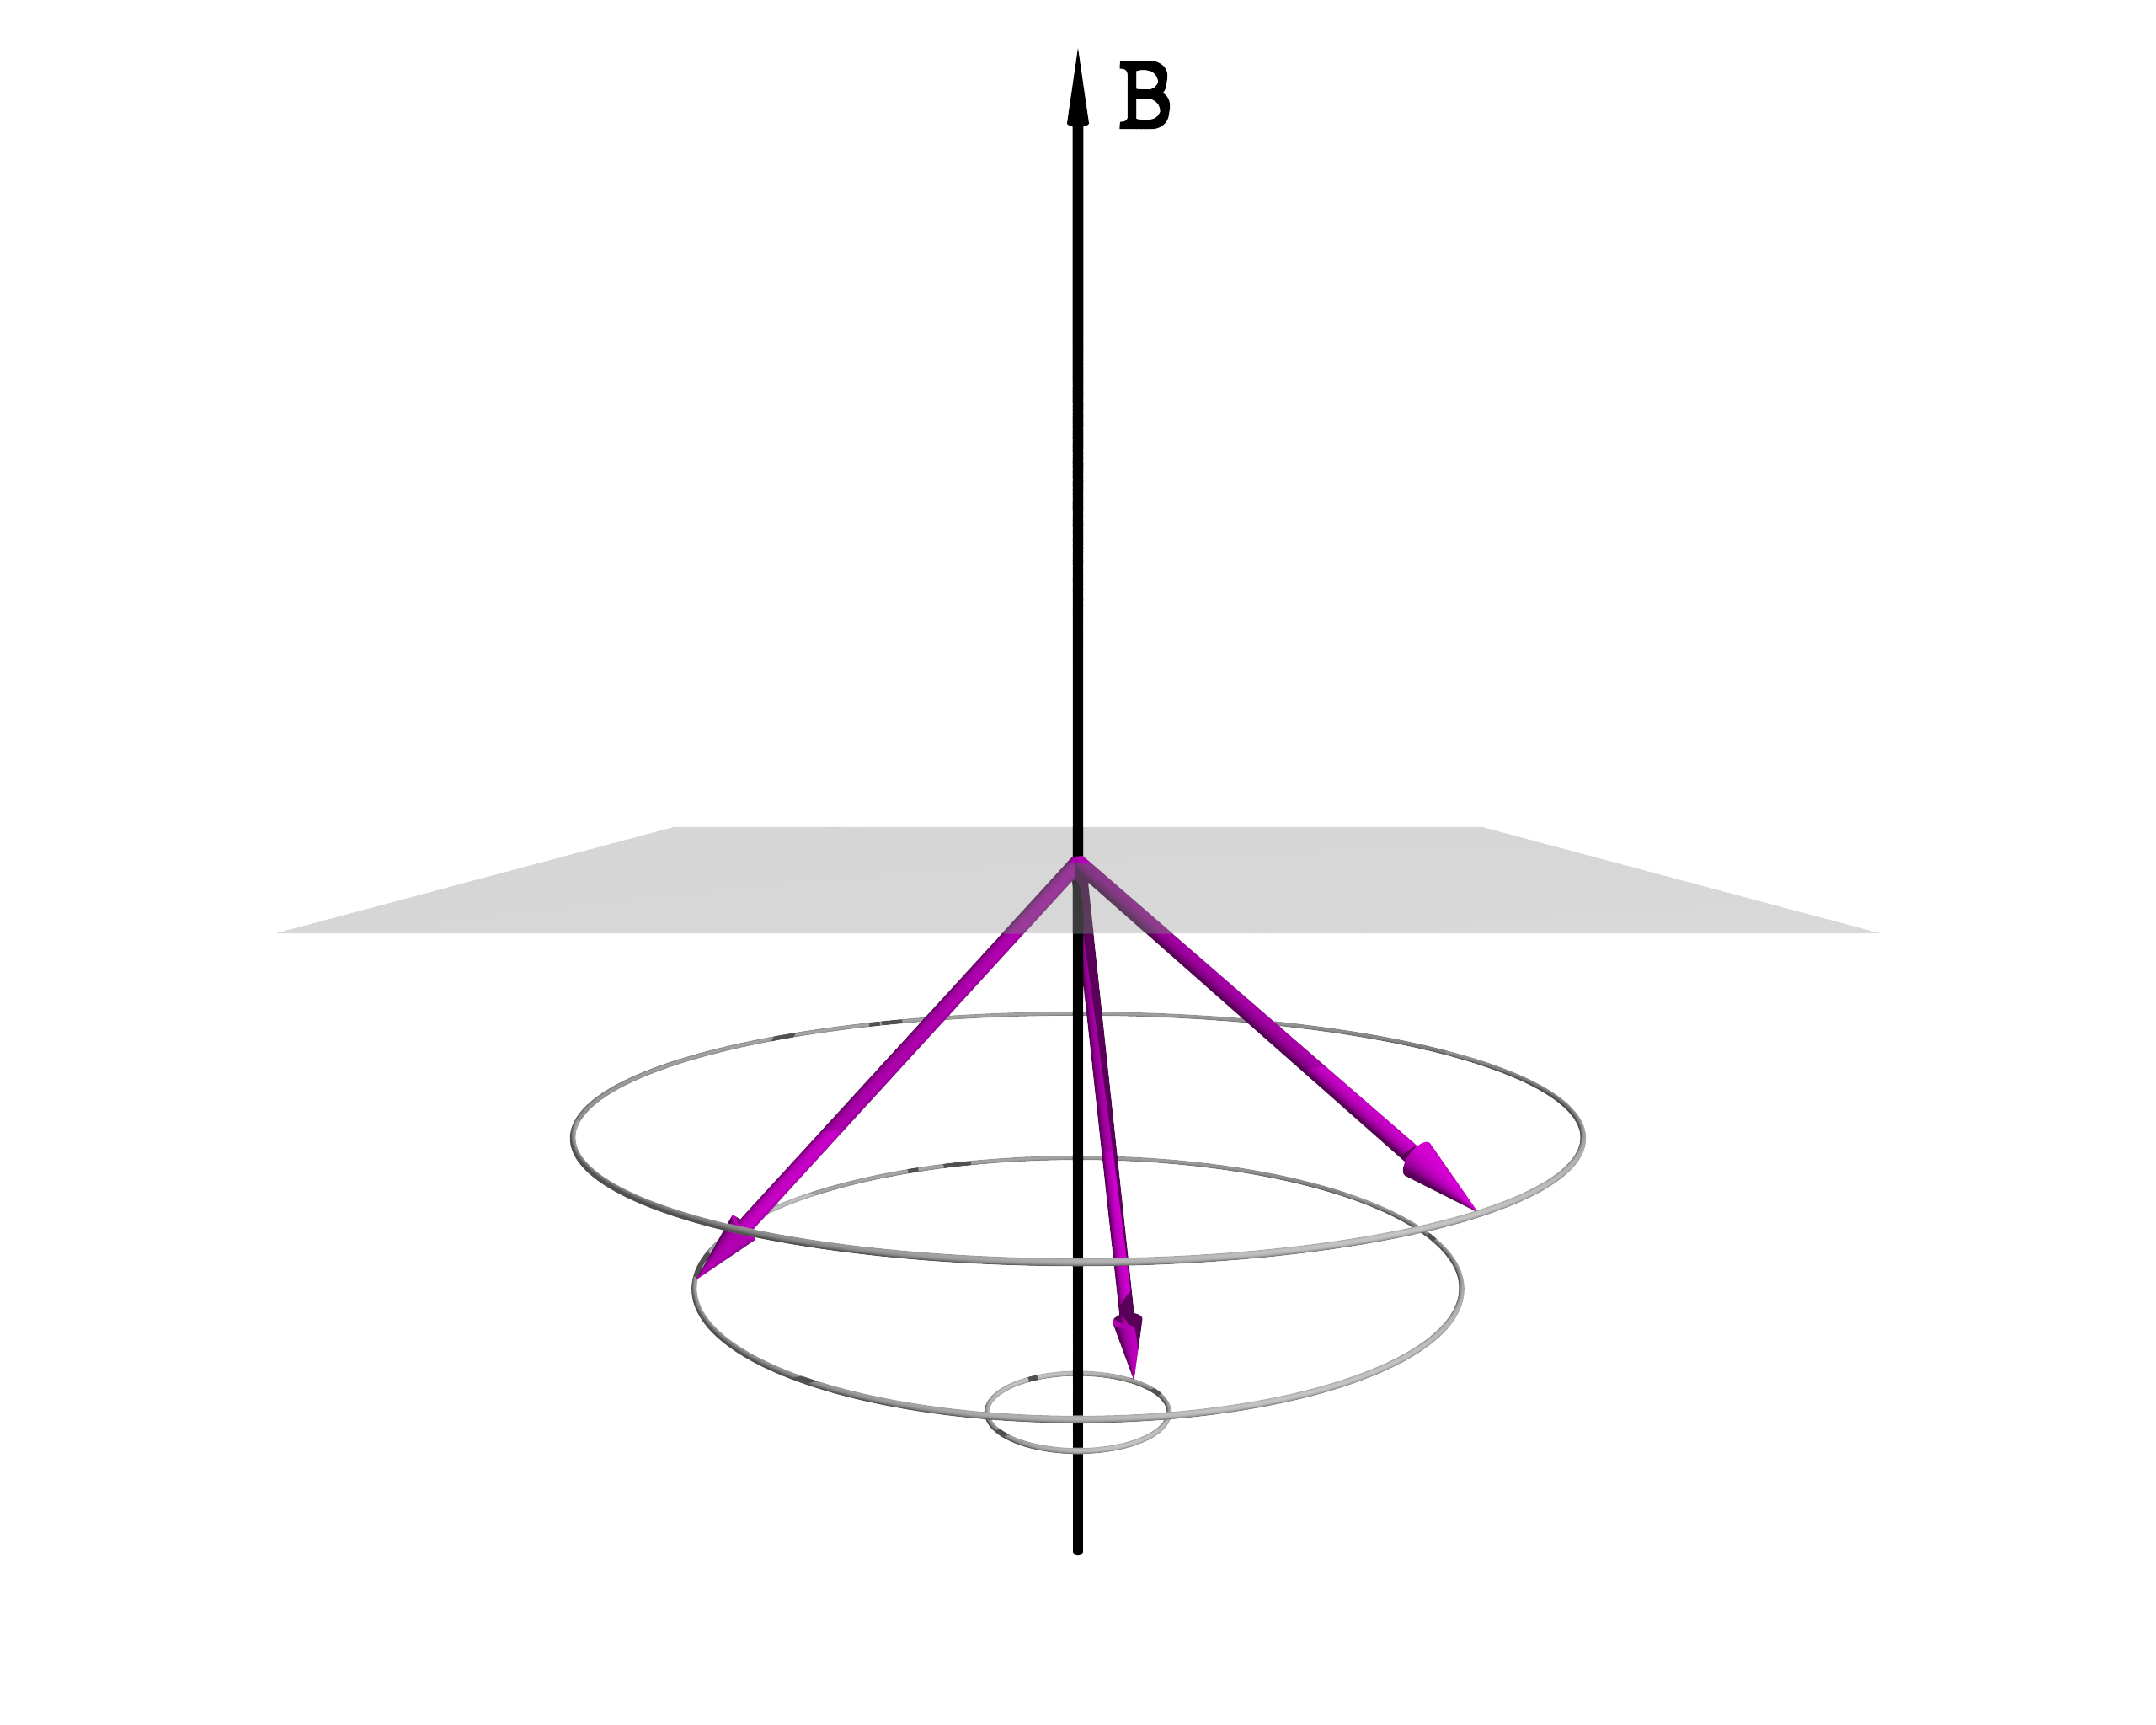
\includegraphics[height=5.5cm]{./mri/pic/Spin2}
		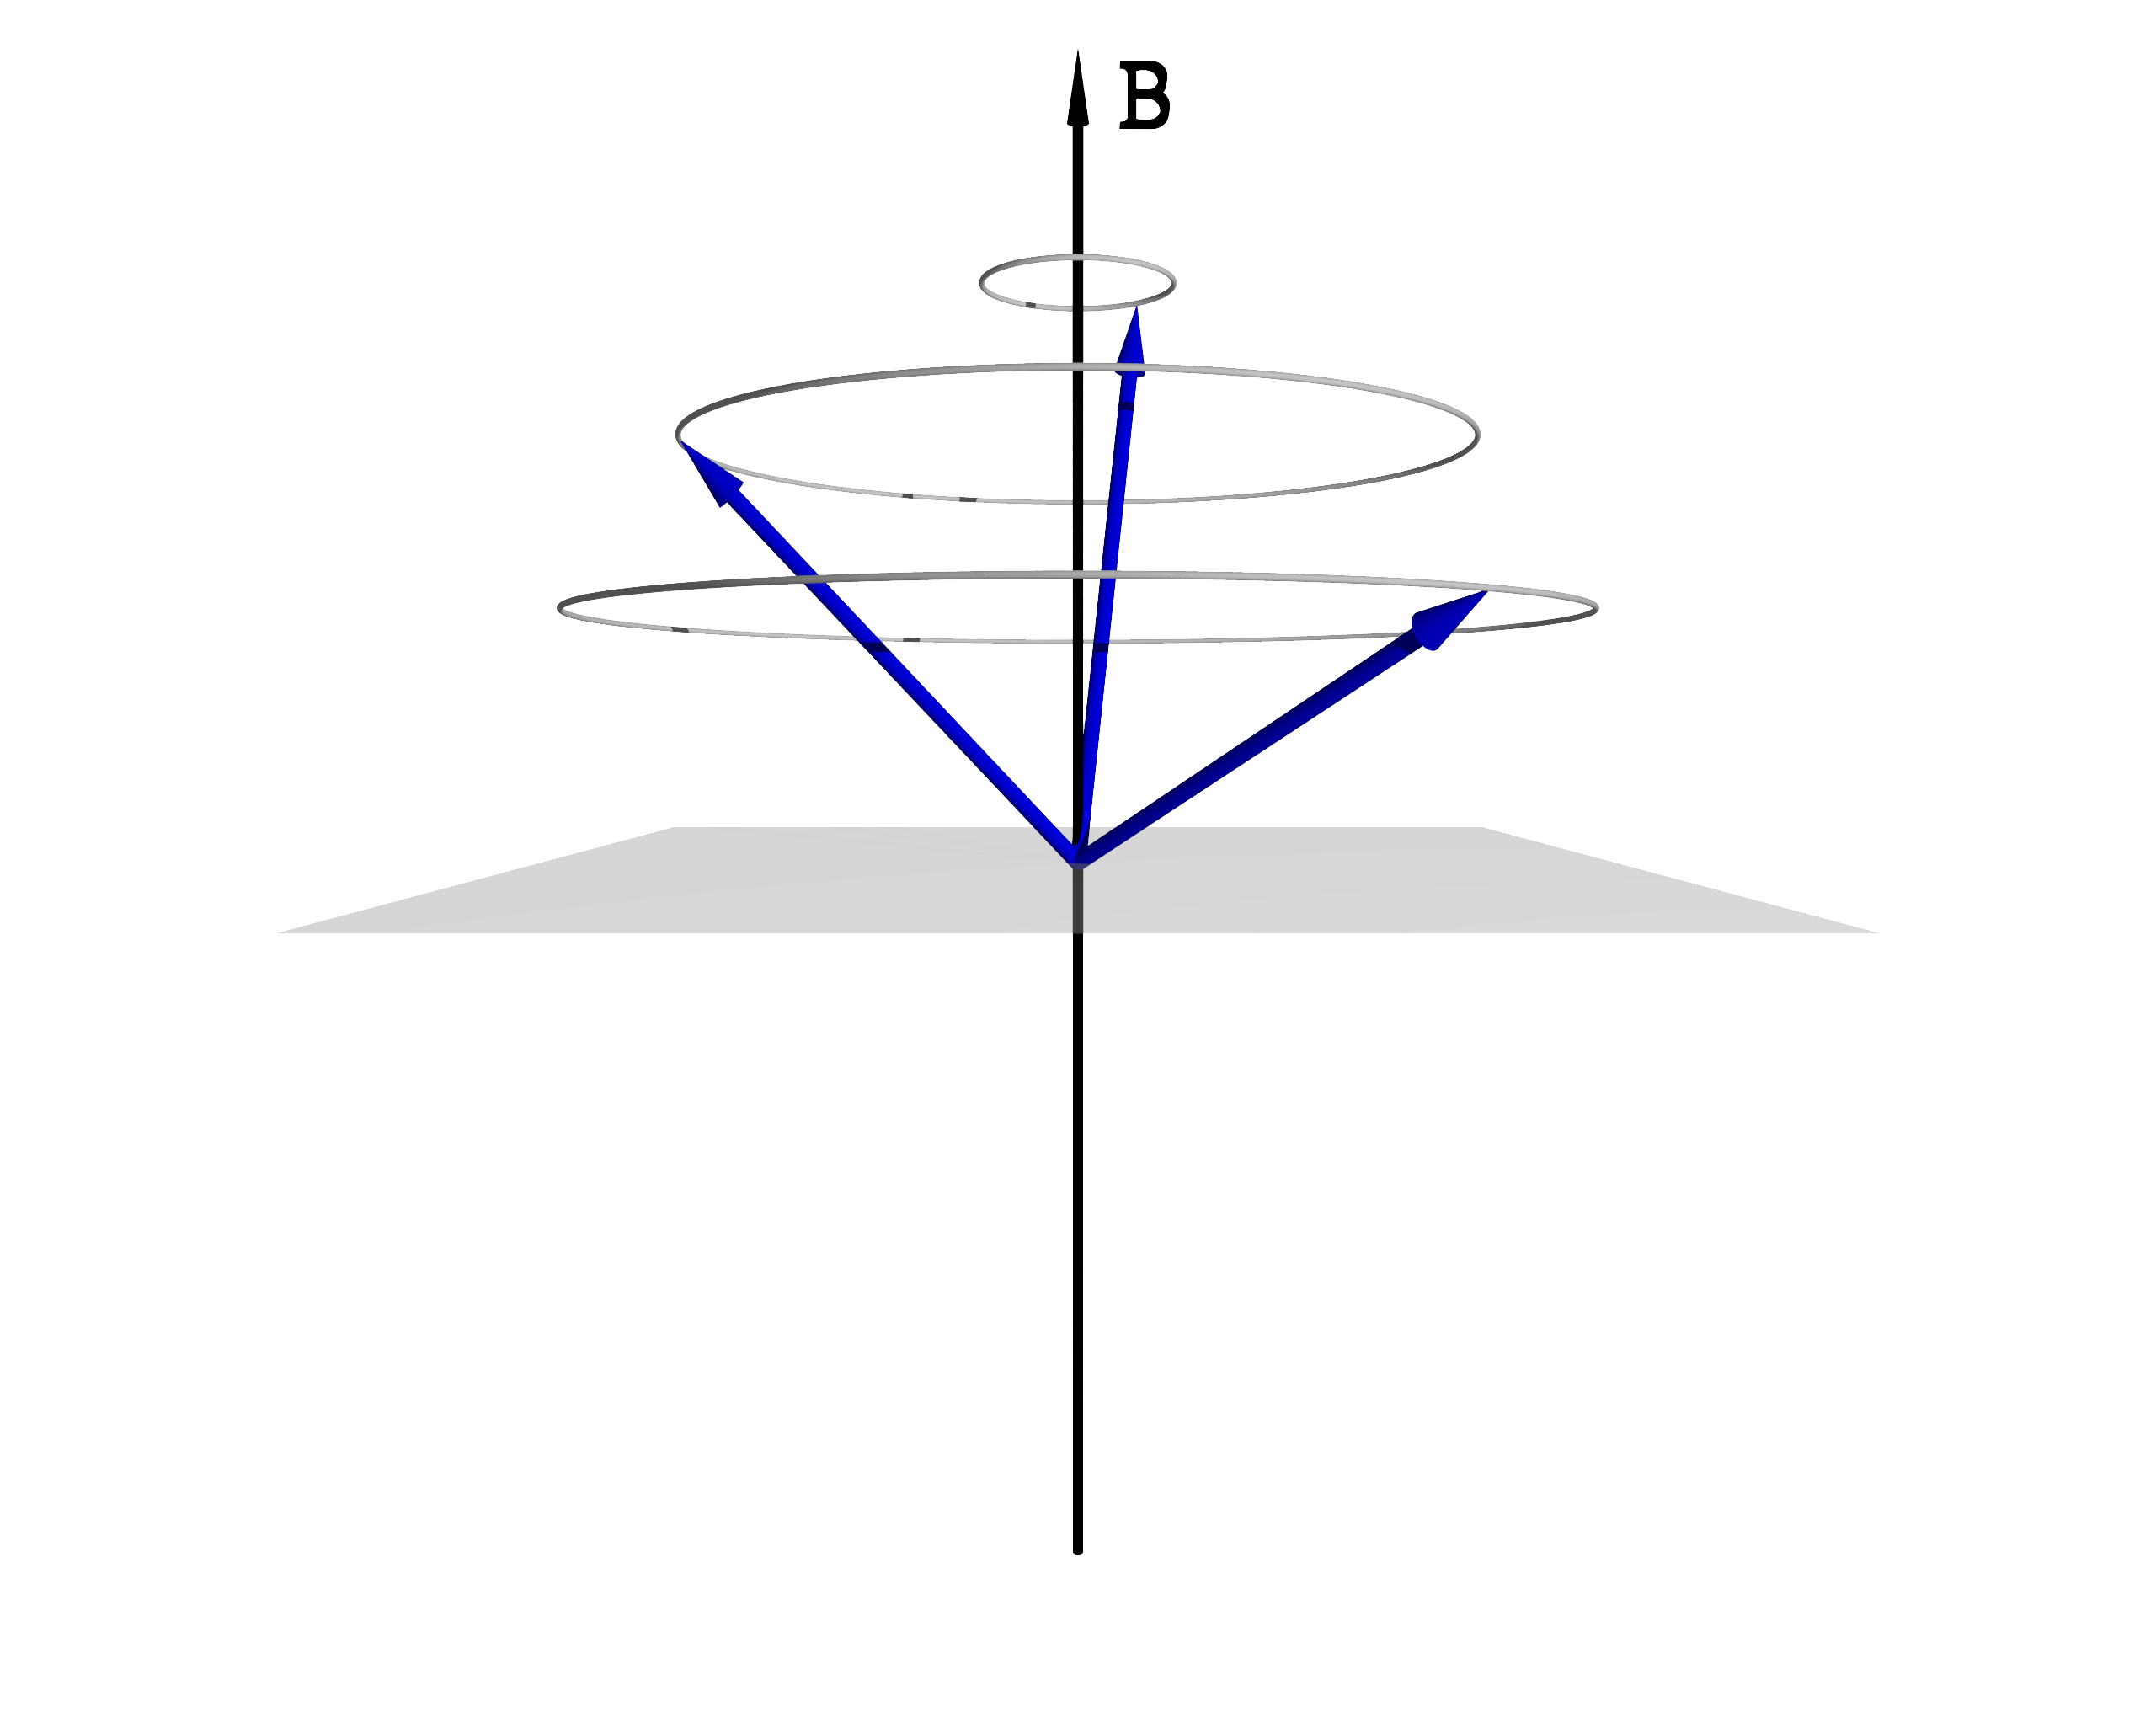
\includegraphics[height=5.5cm]{./mri/pic/Spin1}
		\caption{Links, der energetisch niedrigere Zustand und rechts der h"ohere Zustand. Dabei k"onnen die Winkel $\theta$ innerhalb der Zust"ande alle beliebigen Werte annehmen.}
		\label{fig:spin}
	\end{figure}
	
	Wie in n"achsten Kapitel genauer beschrieben wird, k"onnen zwei Zust"ande identifiziert werden, die klassisch den Situationen in Abbildung \ref{fig:spin} entsprechen. Sie unterscheiden sich durch das Vorzeichen von $-\vec{\mu} \cdot\vec{B}$. Im quantenmechanischen Modell werden dies zwei klar unterscheidbare Zust"ande mit unterschiedlichen Energien sein.
	
	\subsection{Hochfrequenzimpuls}
	
	Damit die Protonendichte gemessen werden kann, m"ussen die Protonen zum Strahlen angeregt werden. Dies ist mit einem Hochfrequenzimpuls mit Larmorfrequenz m"oglich. Durch einen solchen Impuls werden zwei Effekte erzielt:
	

	
	\begin{enumerate}
		\item Alle Protonen pr"azedieren in Phase. Bildlich kann man sich das Hochfrequenzfeld als ein sich rotierenden Magneten vorstellen. Diese Rotation bringt alle Dipolmomente der Protonen in Phase.
		\item Alle Protonen werden in den gleichen, energetisch h"oheren Zustand gebracht (Abbildung \ref{fig:spin} rechts).
	\end{enumerate}
	
	Dadurch, dass die Protonen in Phase pr"azidieren, erzeugen sie ein messbares Magnetfeld $\vec{M}_{XY}$ senkrecht zum Magnetfeld $\vec{B}_0$. Jedes dieser Protonen hat auch vorher schon ein Magnetfeld $\vec{M}_i$ erzeugt, welche jedoch wegen der destruktiver Interferenz nicht messbar waren.
	
	Weil sich nun alle Protonen im gleichen Zustand befinden, ist ein weiteres Magnetfeld $\vec{M}_{Z}$, das die selbe Ausrichtung wie das Magnetfeld $\vec{B}_0$ hat, messbar. Auch diese Magnetfelder war bereits vorhanden, hat sich aber ebenfalls aufgehoben, weil die beiden Zust"ande gleich stark waren.
	
	Kurz nach dem Impuls wollen die Protonen jedoch wieder in ihren Ausgangszustand zur"uck. Die Zeit die sie dazu ben"otigen wird durch die Zeitkonstante $T_1$ beschrieben.
	
	Aufgrund von kleinen Unregelm"assigkeiten im Magnetfeld, geraten die Protonen ausser Phase. Dieser Prozess ist langsamer als der Vorherige und wird mit der Zeitkonstante $T_2$ beschrieben.
	
	\subsection{Messgeometrie}

	\begin{figure}
		\centering
		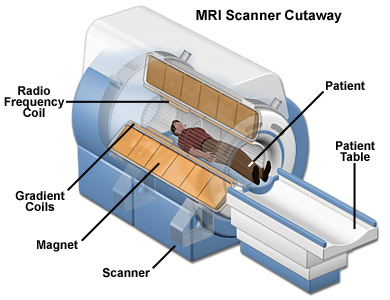
\includegraphics[width = 6cm]{./mri/pic/mri_scanner.jpg} 
		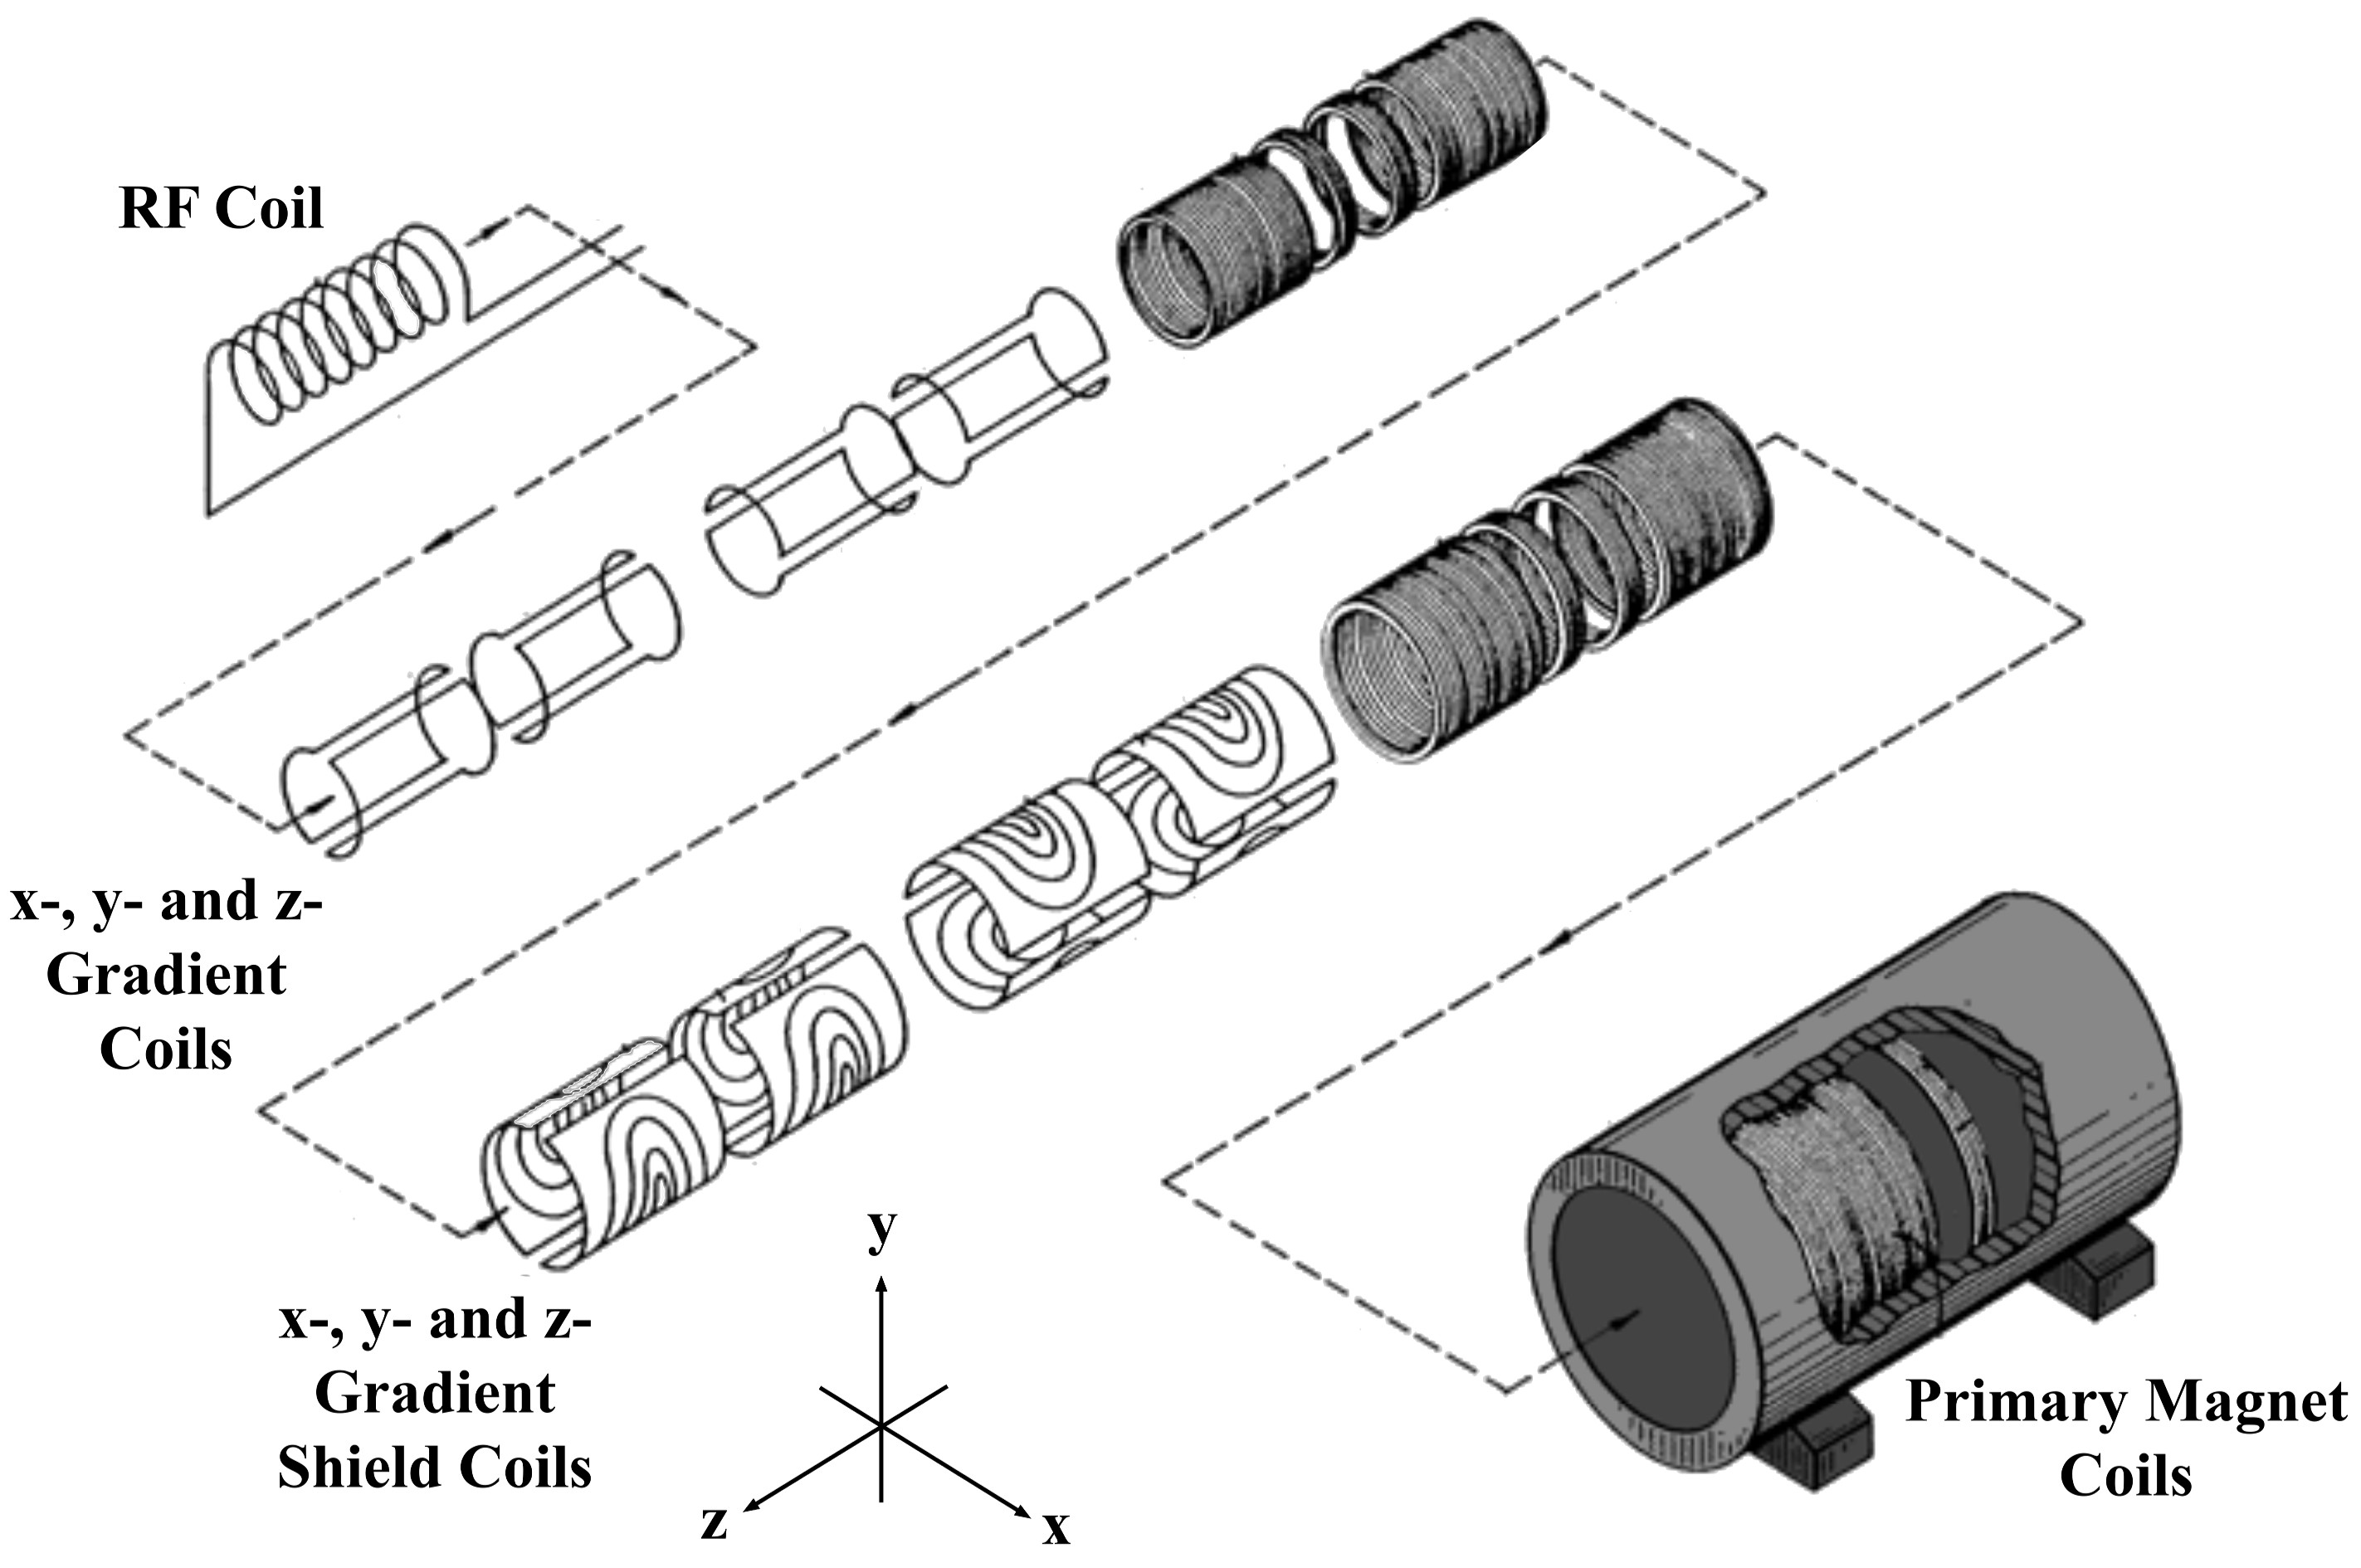
\includegraphics[width = 6cm]{./mri/pic/gradientfield.png}
		\caption{Links die Hauptbestandteile eines MRI-Scanners und rechts die Zusammensetzung der verschiedenen Spulen \cite{MRIScanner}\cite{gradients}.}
		\label{fig:MRIScanner}
	\end{figure}

	Ziel ist es, anhand verschiedenen Messungen der Protonendichte aus verschiedenen Winkeln und Abst"anden, ein Bild zu erzeugen. Dazu wird ein inhomogenes Magnetfeld benutzt, dessen St"arke in eine Richtung zunimmt. Mit der richtigen magnetischen Flussdichte und der dazugeh"origen Frequenz werden die Protonen angeregt. 
	
	Mit Hilfe von Gradientenspulen (Abbildung \ref{fig:MRIScanner} links) wird ein Magnetfeld erzeugt, das in einer Ebene konstant ist. Der anschliessende Hochfrequenzimpuls regt die Protonen dieser Ebene an. Dazu wird eine schmalbandige Spule ben"otigt, in Abbildung \ref{fig:MRIScanner} links, als RF-Spule (engl. \emph{Radio Frequency}) angeschrieben. Die Protonen emittieren kurz nach der Anregung Strahlung, die mit der selben Spule gemessen werden kann.
	
	Aus den verschiedenen Ebenen, die vom Winkel und von der Position abh"angig sind, kann mit der Radon-Transformation \cite{Mathsem} ein Bild berechnet werden.
	

%\section{Grundlagen}
%
%In diesem Abschnitt soll das Prinzip des MRI mit Hilfe der klassischen Physik erkl"art werden. Auf die quantenmechanischen Eigenschaften wird in Abschnitt \ref{sec:quant} eingegangen. Um das MRI Verfahren besser beschreiben zu k"onnen, wird das Modell eines Protons benutzt.
%
%\subsection{Magnetismus}
%
%%TODO
%%Um das MRI Verfahren zu verstehen ist es wichtig, dass der Magnetismus verstanden wurde. An dieser Stelle werden noch einmal die wichtigsten Eigenschaften erl"autert.
%Um das MRI Verfahren zu verstehen ist es wichtig, dass die Grundlagen des Magnetismus verstanden wurden. An dieser Stelle werden noch einmal die wichtigsten Eigenschaften erl"autert.

%verschiedene Magnetfeldst�rken, bis 0.5 Tesla Permanentmagnete
%
%\section{Grundlagen}
%
%\subsection{Magnetismus}
%
%\subsection{Pr�zession}
%
%\begin{figure}
%	\centering
%	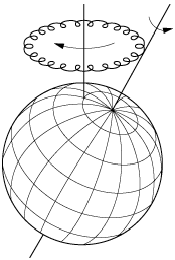
\includegraphics[height=4cm]{./mri/pic/praezession}
%	\caption{Pr�zession \cite{praezession}}
%	\label{fig:spin}
%\end{figure}
%
%\subsubsection{Larmor-Pr�zession}
%
%
%
%\subsection{NMR -- Nuclear Magnetic Resonance}
%
%\subsection{MRI Signal}


%Jeder Magnet erzeugt in sich geschlossene Feldlinien. Sie f"uhren vom magnetischen Nordpol zum magnetischen S"udpol. Auch jeder mit elektrischem Strom durchgeflossene Leiter erzeugt ein magnetisches Feld (Abbildung \ref{fig:magnetismus}). Dabei wird die elektrische Feldst"arke $H$ oder die magnetische Flussdichte $B$ angegeben \cite{wiki:magnetismus}.
%
%\begin{figure}
%	\centering
%	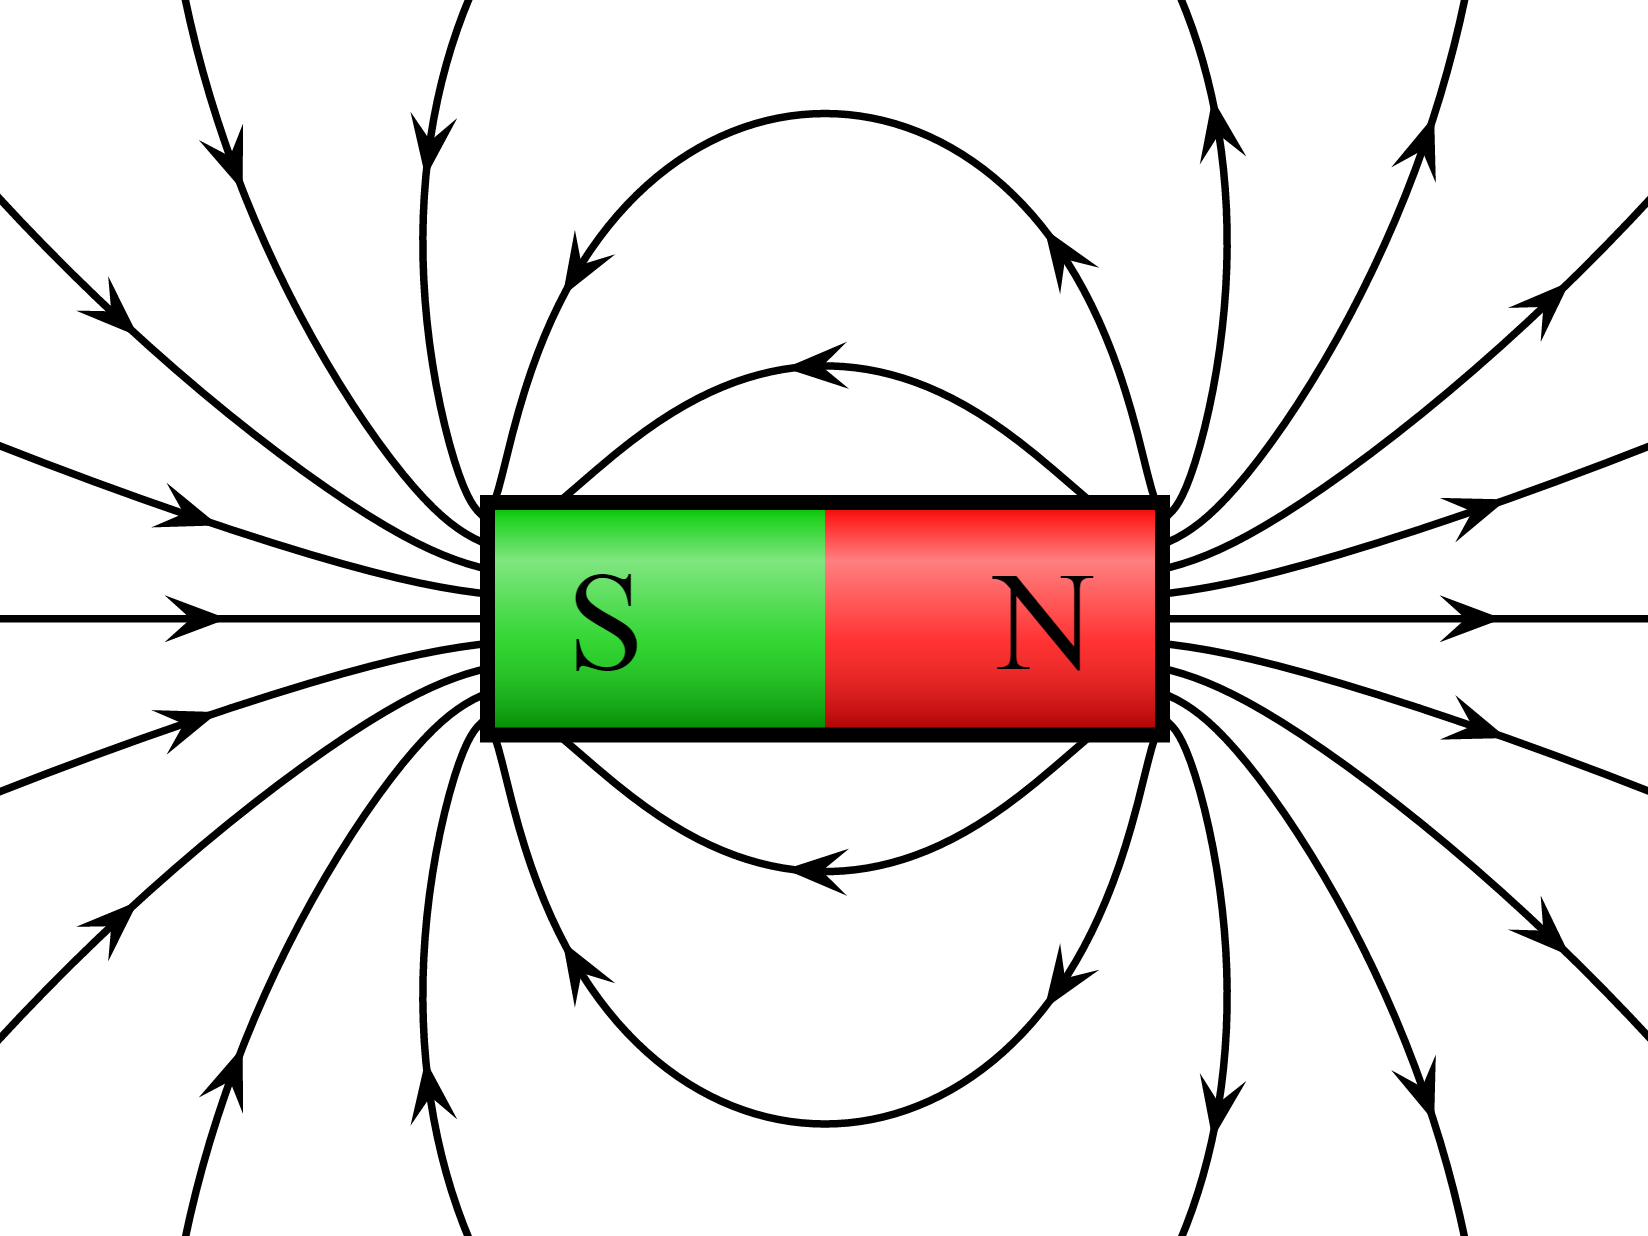
\includegraphics[height=2.5cm]{./mri/pic/mag1}
%	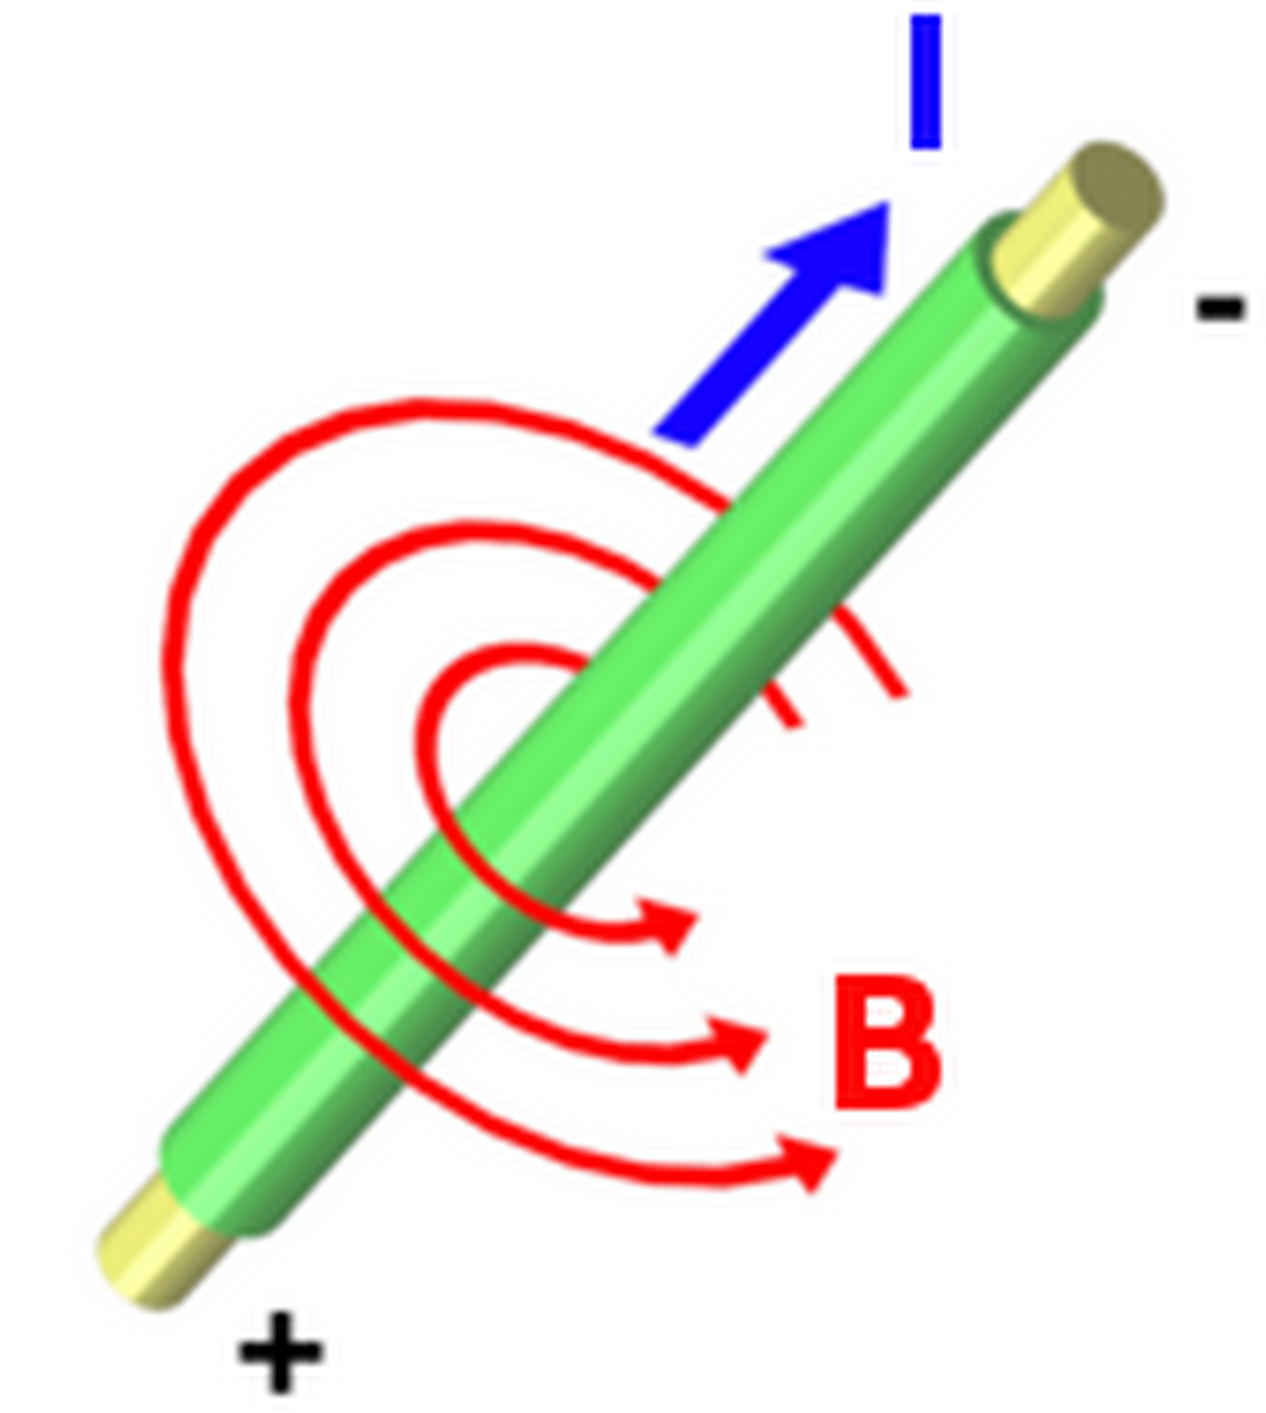
\includegraphics[height=2.5cm]{./mri/pic/mag2}
%	\caption{Magnetismus: Links ein Stabmagnet, der mit in sich geschlossenen Feldlinien umgeben ist. Rechts ein Leiter der mit elektrischem Strom durchflossen ist. \cite{wiki:magnetismus}}
%	\label{fig:magnetismus}
%\end{figure}

%\subsection{Pr"azession}
%
%Ein einfaches Modell eines Protons ist ein Stabmagnet. Der Nord- und der S"udpol dieses Magneten liegen nicht perfekt auf einer Linie mit der Rotationsachse des Protons. Die Rotationsachse taumelt, was als Pr"azession bekannt ist (Abbildung \ref{fig:praezession}). Eine Analogie da zu ist ein Kreisel, der immer langsamer wird und beginnt zu taumeln. 
%Die Frequenz, mit der sich das Proton um die Achse des Magnetfeld dreht, ist $\omega_p$. Sie ist nicht mit der Frequenz der Drehung des Protons selber zu verwechseln.
%
%\begin{figure}
%	\centering
%	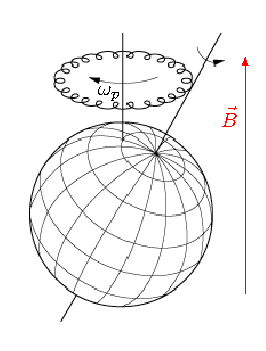
\includegraphics[height=5cm]{./mri/tikz/precession}
%	\caption{Pr"azession: Modell eines Protons das sich in einem Magnetfeld $\vec{B}$ befindet,  \cite{praezession}}
%	\label{fig:praezession}
%\end{figure}
%
%
%
%\subsection{NMR -- Nuclear Magnetic Resonance }\label{mri:grundlagen:NMR}
%
%\begin{figure}
%	\centering
%	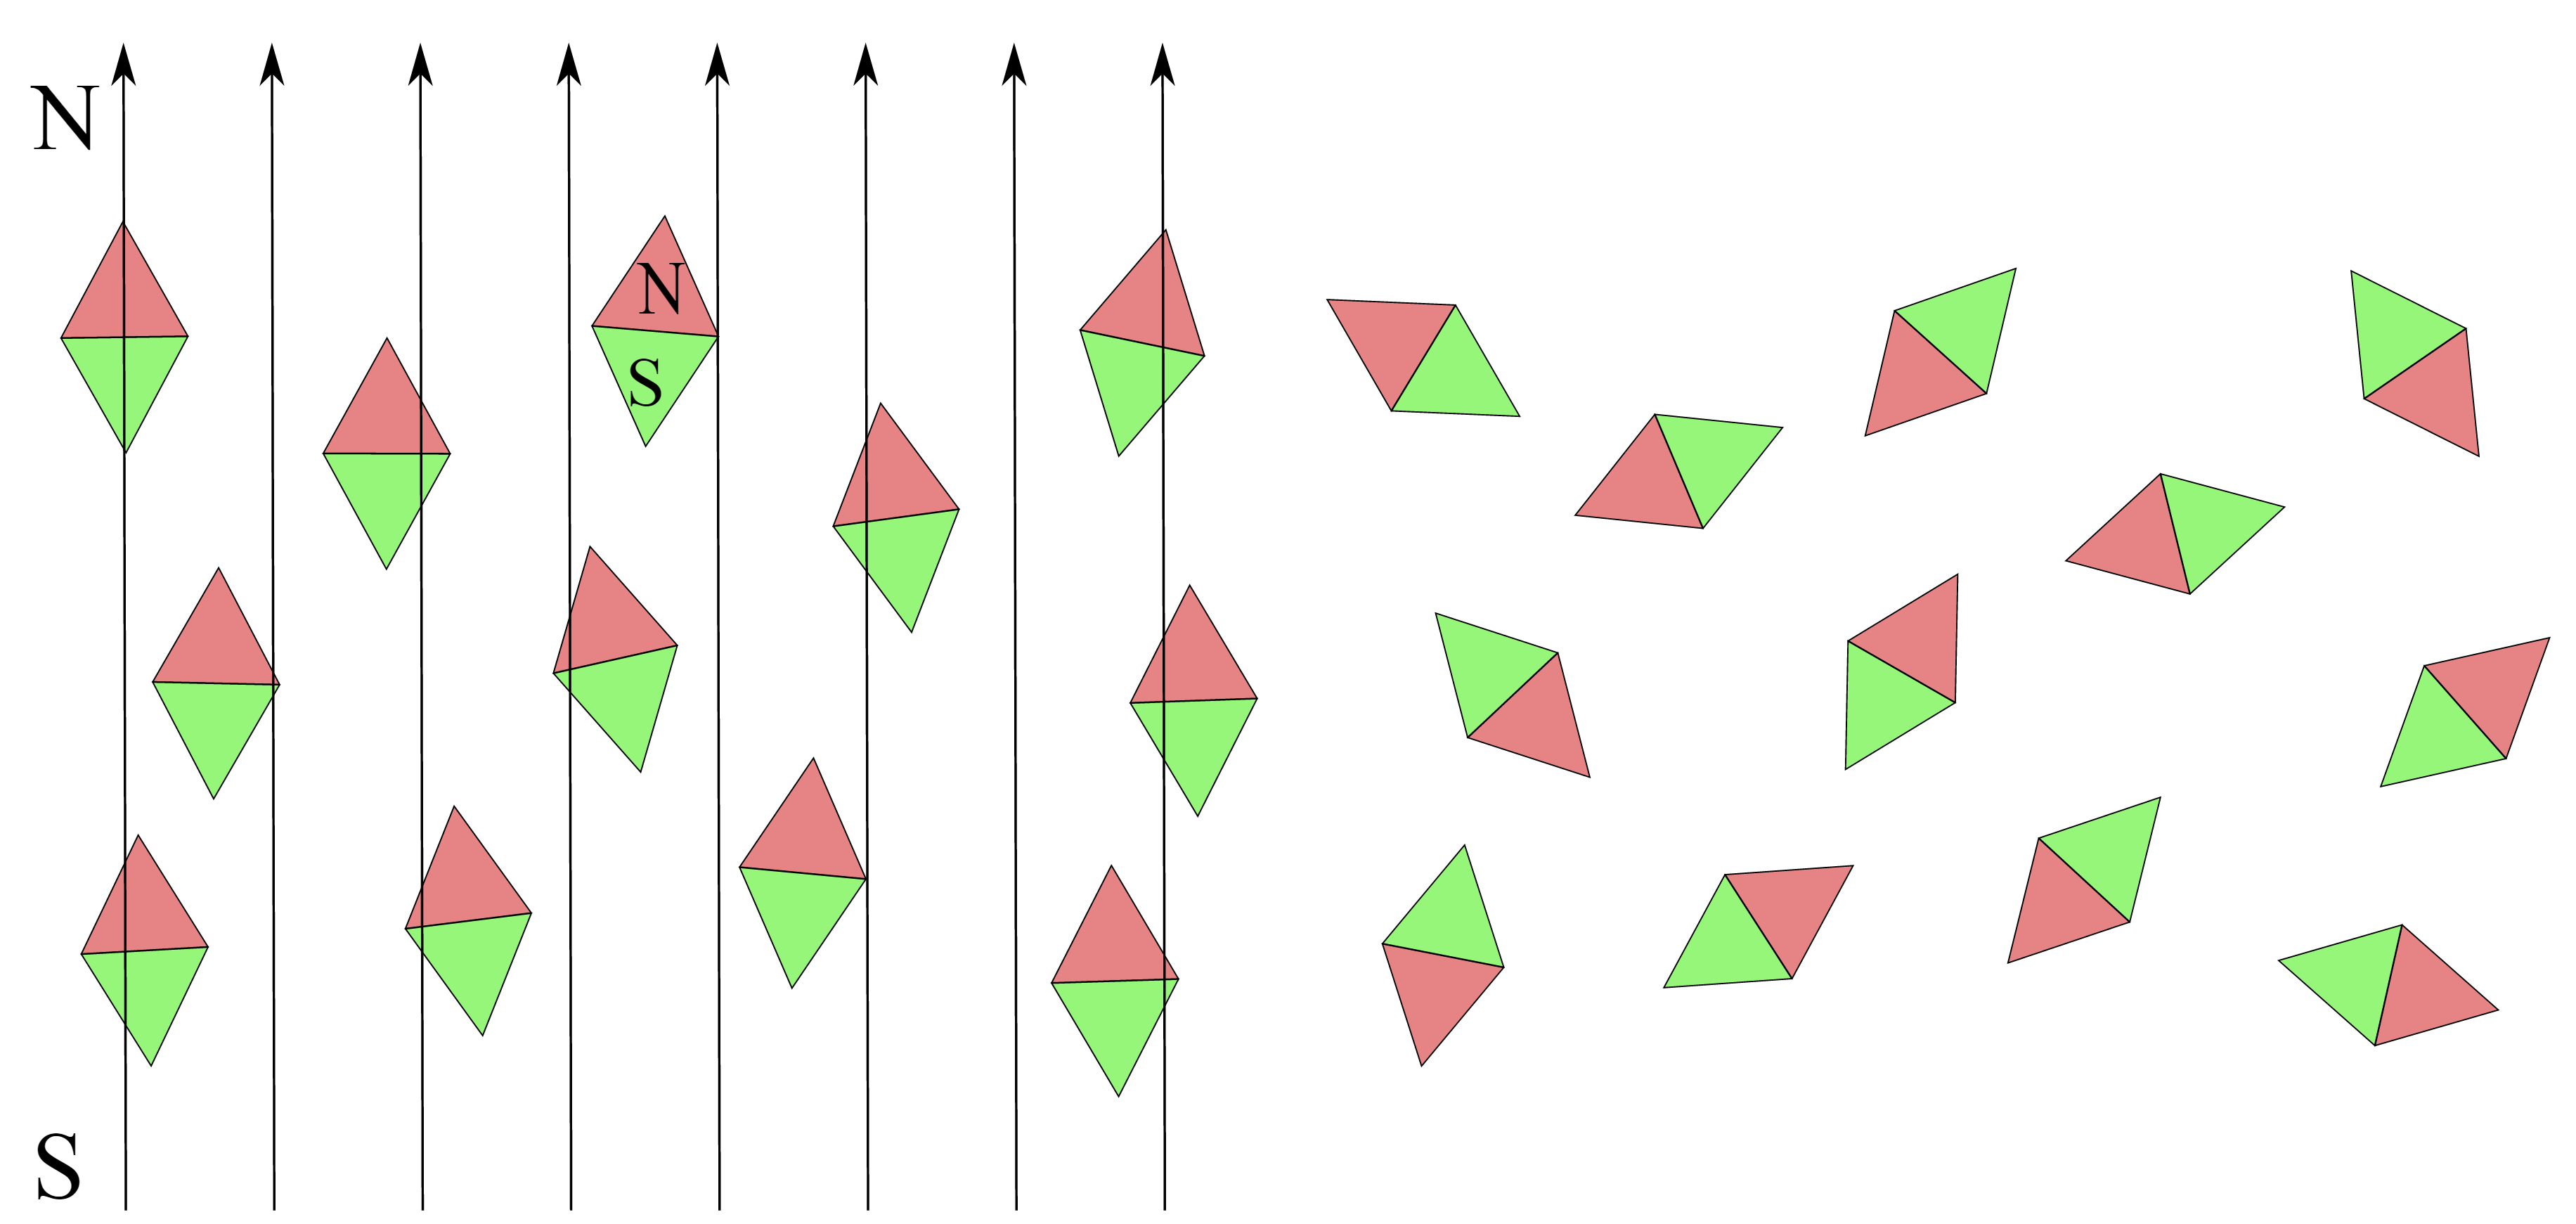
\includegraphics[height=4cm]{./mri/pic/mag3}
%	\caption{Links: Mehrere Protonen, als Stabmagnete gezeichnet, richten sich dem Magnetfeld aus. Rechts: Protonen im Ausgangszustand \cite{wiki:magnetismus}}
%	\label{fig:magnetismus2}
%\end{figure}
%
%Wenn nun mehrere solche Protonen mit einem statischen Magnetfeld angeregt werden, richten sich diese aus. Dabei gibt es zwei Zust"ande: Den stabilen Zustand, indem sich die Protonen parallel zum Magnetfeld ausrichten. Dabei ist die Polarisierung des externen Magnetfelds und die des Protons N--S--N--S. Im zweiten, instabilen Zustand, ist die Ausrichtung N--N--S--S und damit energetisch h"oher, die Protonen richten sich anti-parallel aus, also um 180$^{\circ}$ gedreht (Abbildung \ref{fig:magnetismus2} links). 
%
%Die Protonen k"onnen vom niedrigeren Zustand in den h"oheren Zustand wechseln in dem sie ein Photon absorbieren. Wenn sie den Zustand erneut wechseln, geben sie ein Photon ab. Die Energie $E$ des Photons muss dabei exakt stimmen, damit ein Wechsel m"oglich ist. Die Energie des Photons ist von dessen Frequenz $f$ und von der Planck'schen Konstanten $h$ abh"angig \cite{MRI:Joseph}.
%\begin{equation}
%E= h\cdot f
%\end{equation}
%Die Frequenz entspricht der Larmorfrequenz $f = f_{Larmor}$
%
%\subsubsection{Bolzmannstatistik}
%
%Wenn sich nun mehrere Protonen in einem Magnetfeld befinden, richtet sich ein Teil parallel, im niedrigieren Zustand $N^{+}$, aus und ein Teil richtet sich anti-parallel, im h"oheren Zustand $N^{-}$, aus. Die Verteilung ist temperaturabh"angig
%\begin{equation}
%\dfrac{N^{-}}{N^{+}}= e^{-E/kT}
%\end{equation}
%$E$ ist die Energiedifferenz zwischen den Spinzust"anden, $k$ ist die Bolzmannkonstate und $ T$ ist die Temperatur in Kelvin.
%
%Jedes Proton erzeugt sein eigenes kleines Magnetfeld $\vec{M}_{Z,i}$, das in der $Z$-Achse liegt. Die Summe all dieser Vektoren ist proportional zu $N^{+}-N^{-}$.
%\begin{equation}
%\displaystyle \sum_{i} \vec{M}_{Z,i} =\vec{M}_Z
%\end{equation}   
%
%\subsubsection{$T_1$ Prozess}
%
%Im Gleichgewicht liegt die Gesamtmagnetisierung $\vec{M}_Z$, auch Longitudinal-Magnetisierung genannt, in Richtung des externen Magnetfeldes $\vec{B}_0$. Sie wird im folgenden $\vec{M}_0$ genannt. In dieser Ausgnagslage gibt es keine Transversal-Magnetisierungen $\vec{M}_X$ oder $\vec{M}_Y$.
%
%Wenn dem System nun genug Energie zugef"uhrt wird, ist es m"oglich, das System zu s"attigen, so dass $\vec{M}_Z=0$. Das System wird aber nach einer gewissen Zeit wieder im Ausgangszustand sein, dabei gibt es Energie, bzw. Photonen ab. Diese Zeit wird durch die Zeitkonstante $T_1$ beschrieben (engl. spin lattice relaxation time).
%\begin{equation}
%{M}_{Z}= M_0\left(1-e^{-t/T_1}\right)
%\end{equation}
%
%\subsubsection{$T_2$ Prozess}
%
%Kurz nachdem das System in den energetisch h"oheren Zustand gebracht wurde, haben alle Protonen die gleiche Pr"azessionsfrequenz und sind phasengleich ausgerichtet. Aufgrund von kleinen Unterschieden im Magnetfeld beginnen sie jedoch aus dem Takt zu geraten und rotieren mit ihrer eigenen Larmorfrequenz. Dabei nimmt die Transversal-Magnetisierung $M_{XY0}$ ab. Diese Zeit wird mit der Zeitkonstante $T_2$ beschrieben (engl. spin-spin relaxation time).
%
%\begin{equation}
%M_{XY}=M_{XY0}e^{-t/T_2}
%\end{equation}
%Es gilt $T_2 \le T_1$. Es treten beide Prozesse, $T_1$ und $T_2$, gleichzeitig auf.
%
%\subsection{RF-Signal}
%
%Eine Spule in Richtung der $X$-Achse wird mit Wechselstrom angeregt (Abbildung \ref{fig:MRIScanner}). Sie erzeugt dabei ein wechselndes Magnetfeld in Richtung der $X$-Achse. Man kann sich das vorstellen, als w"urde sich ein Magnet in der $XY$-Ebene um die $Z$-Achse rotieren. Wenn nun die Frequenz der Rotation mit der Larmorfrequenz "ubereinstimmt, bewegt sich das Magnetfeld der Spule relativ zu dem Protonen nicht.
%
%\subsubsection{MRI Signal}
%
%Wenn nun das alternierende Magnetfeld kurz eingeschaltet und dann wieder ausgeschaltet wird, kann die Relaxation gemessen werden. Dabei kann eine Spule als Sender und Empf"anger genutzt werden, weil das Empfangssignal die gleiche Frequenz wie das Sendesignal hat. Dieser gesendete Impuls ist k"urzer als $T_2$. Weil sich diese Frequenzen dieser Signales im Hochfrequenzbereich befinden werden sie als RF-Signale bezeichnet (engl. RF: Radio Frequency).
%
%\subsection{Das statische Magnetfeld}
%
%\begin{figure}
%	\centering
%	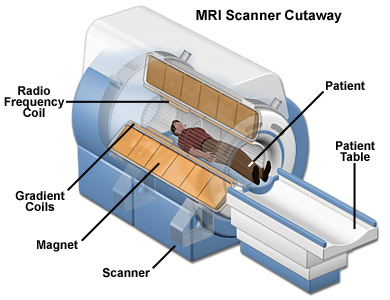
\includegraphics[width = 6cm]{./mri/pic/mri_scanner.jpg} 
%	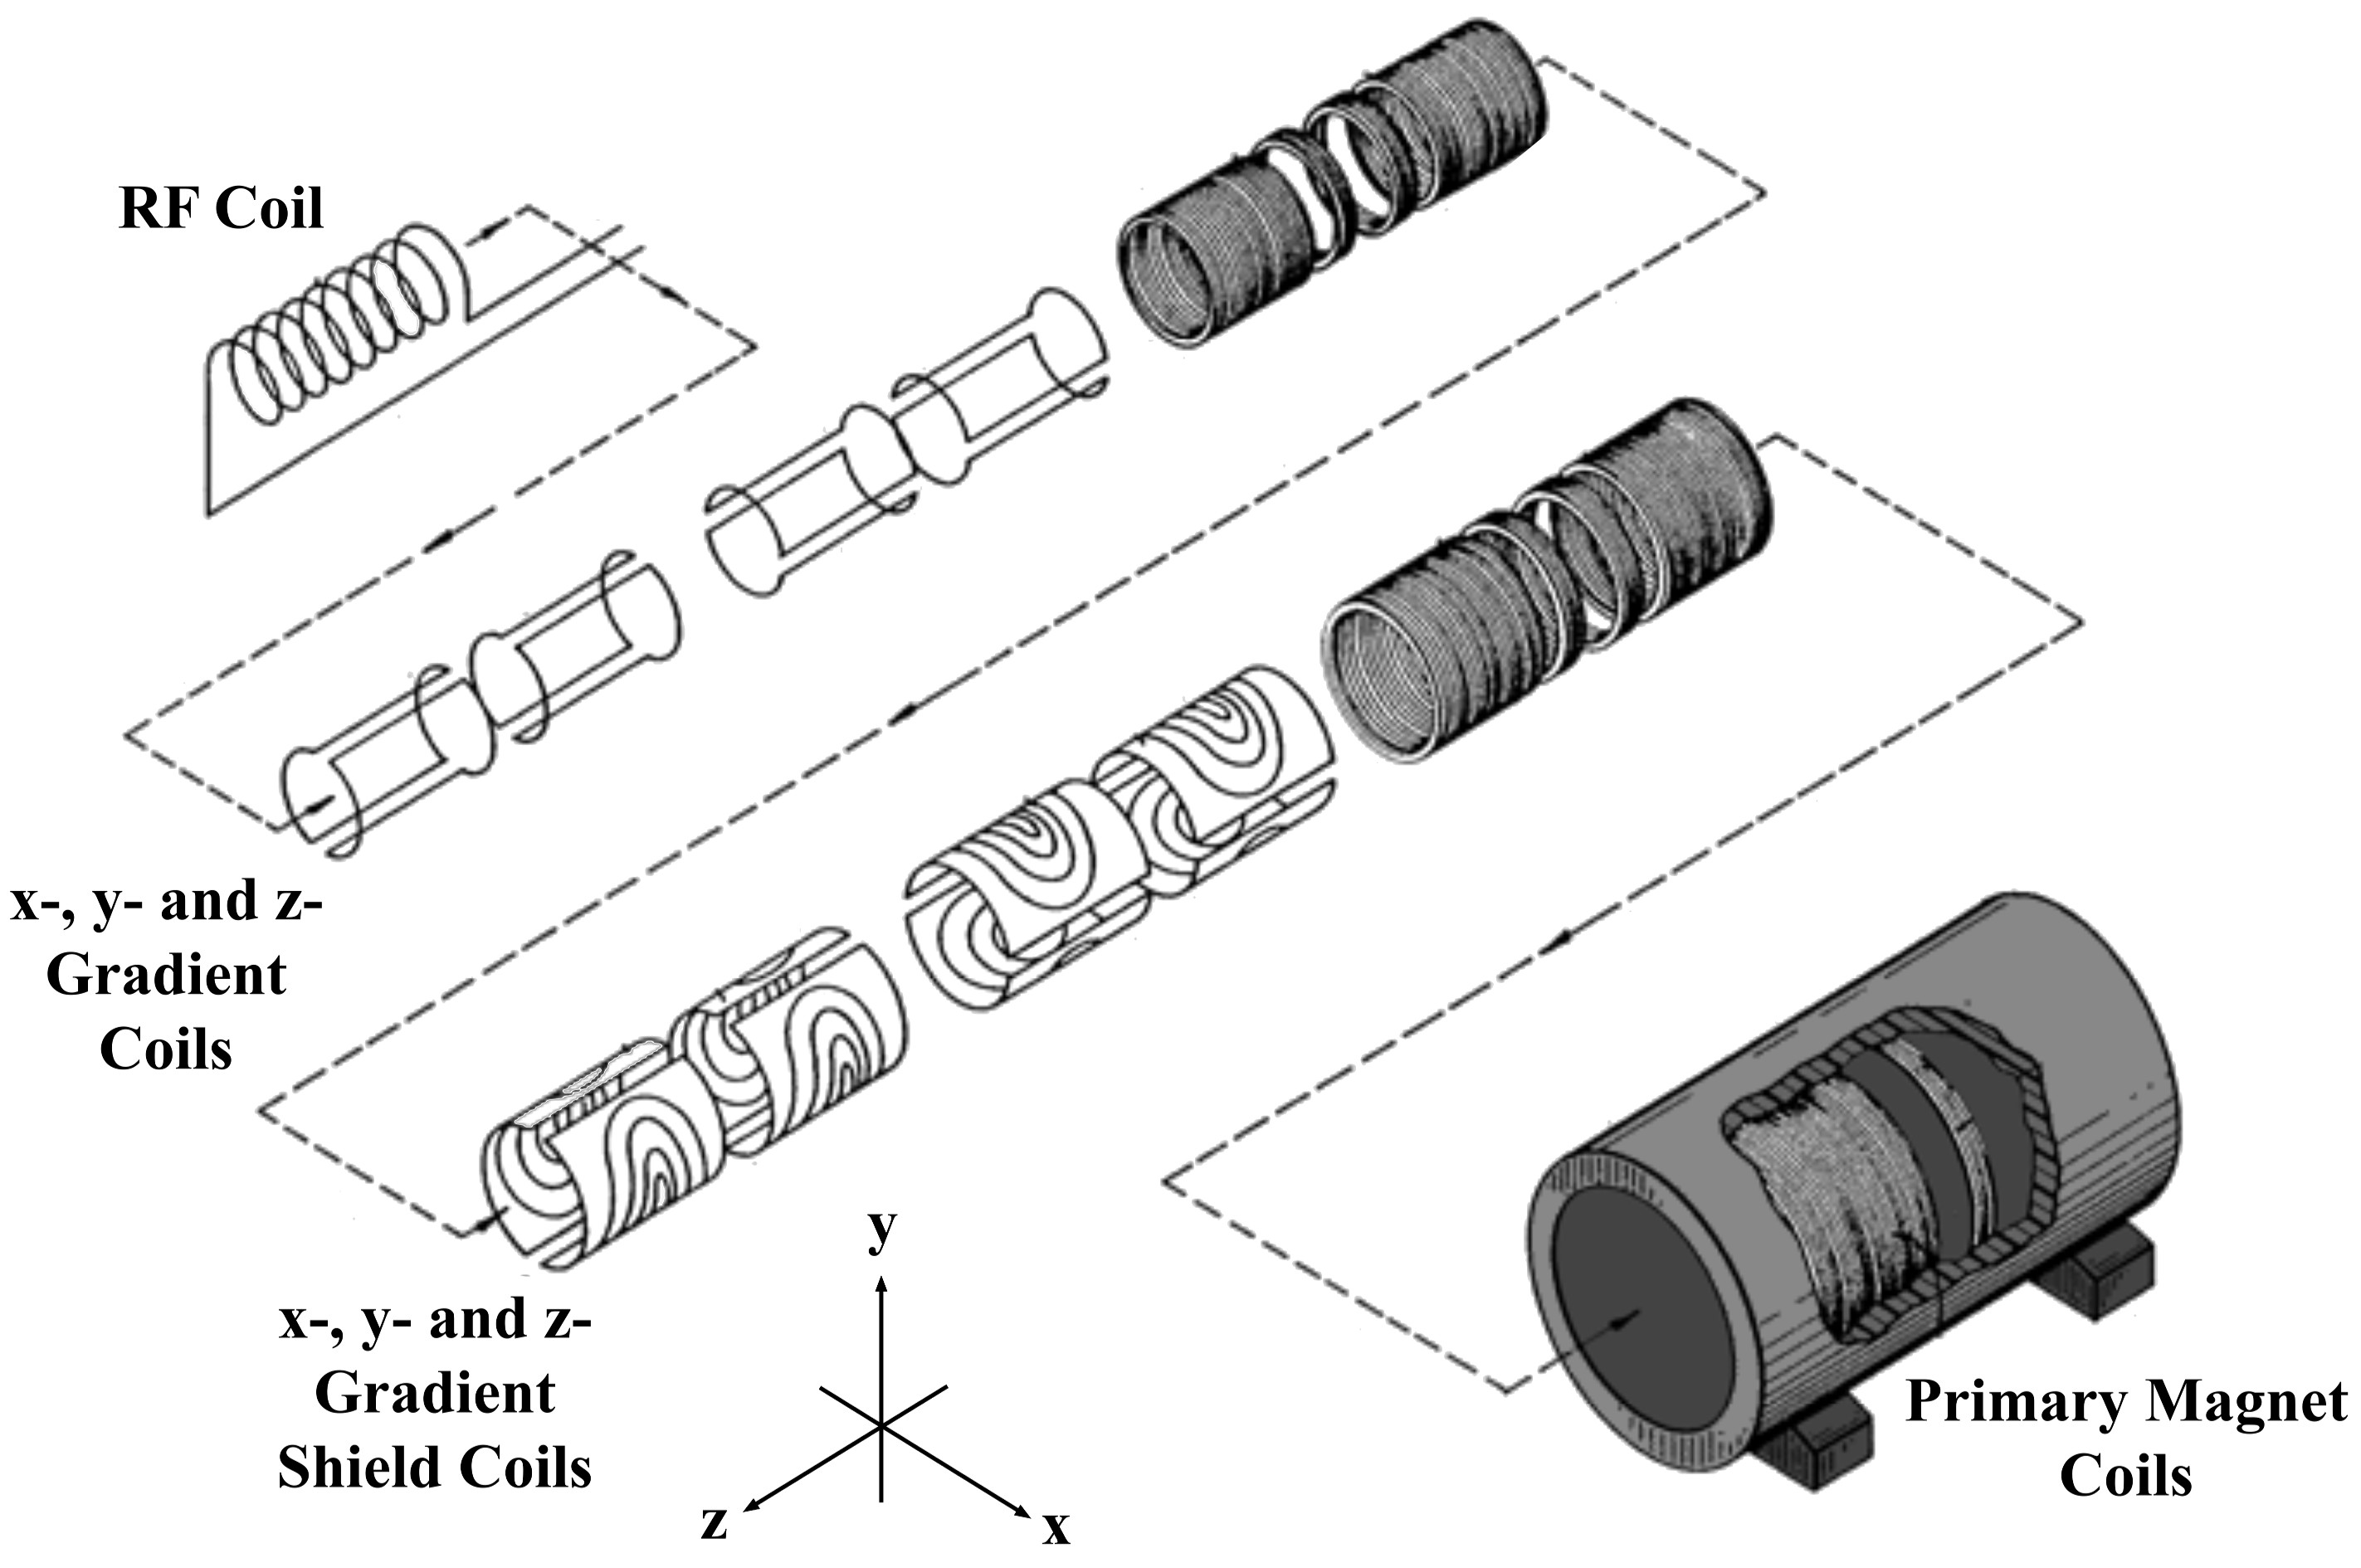
\includegraphics[width = 6cm]{./mri/pic/gradientfield.png}
%	\caption{Links die Hauptbestandteile eines MRI-Scanners und rechts die Zusammensetzung der verschiedenen Spulen \cite{MRIScanner}\cite{gradients}.}
%	\label{fig:MRIScanner}
%\end{figure}
%
%Eine wichtige Voraussetzung f"ur die Magnetresonanztomographie ist das statische Magnetfeld, welches hohe Anspr"uche erf"ullen muss. 
%Die Homogenit"at und die zeitliche Stabilit"at sind essenziell. 
%Medizinische Apparaturen arbeiten "ublicherweise mit 0.5 bis zu 3 Tesla. Neuere Ger"ate k"onnen Flussdichten bis zu 7 Tesla erreichen, daf"ur sind aber supraleitende Magnetspulen notwendig.
%
%\subsection{Das Gradientenfeld}
%
%Gem"ass Gleichung \ref{eq:larmorf} schwingen nur jene Teilchen mit $f_{Larmor}$, die der Flussdichte $B_0$ ausgesetzt sind. Um einen gew"unschten Bereich messen zu k"onnen, ist dem statischen homogenen Magnetfeld ein schw"acheres inhomogenes Gradientenfeld "uberlagert, dieses wird mit mehreren Magneten erzeugt.
%Die Gradientenfeld ist von der Position abh"angig. Ein eindimensionaler Feldgradient hat eine "Anderung das Magnetfeldes in einer Richtung. Dieser ist auch der Wichtigste.



